% !TeX spellcheck = en_GB
%-------------------------------------------------------------------------------
% File: simulation.tex
%       Vehicle ADVISE project documentation.
%
% Author: Yuri Mazzuoli, Francesco Iemma, Marco Pinna
%         Created on 30/06/2021
%-------------------------------------------------------------------------------
\chapter{Simulation}\label{ch:simulation}

We implemented the attack tree in Mobius Tool in order to get some insights about the
attackers behaviour and the most dangerous attack paths. 
We took an heuristic approach in order to evaluate cost and duration of different attacks; the time unit for attacks is \textit{hours}.
\section{General Results}
We decided to simulate 200 units of time (200 h) with Mobius in order to evaluate each attacker's results for 
different configuration of mitigations. The following general results were obtained:\\
\begin{itemize}
    \item the \textbf{Hacker} will always try to achieve the most remunerative goals, despite the
        possibility to be detected; 
    \item the \textbf{Physical intruder} will try to achieve only the most remunerative goal, and will
        ignore the others because of the high probability of being detected (reward-risk ratio is too low)
    \item the \textbf{Insider} has the same behaviour as the Physical intruder, but for them the probability
        to reach the goal increases faster because their attack path has a higher success probability.
\end{itemize}
\newpage
\section{Hacker Attacks}
\subsection*{DoS}
When no mitigations are applied, the Hacker will rarely try to obtain a DoS, but they will commit themselves
to other attacks in order to obtain high reward goals. Introducing \textbf{CodeObfuscation}, binary reversing
become harder to complete with success, leading to a probability of reaching the DoS goal near to 0.\\
Increasing the firewall sensitivity will indeed increase the probability for the hacker to reach the DoS,
because they will give up on trying to reach other goals, focusing only on this one.
\begin{figure}[H]
    \begin{center}
        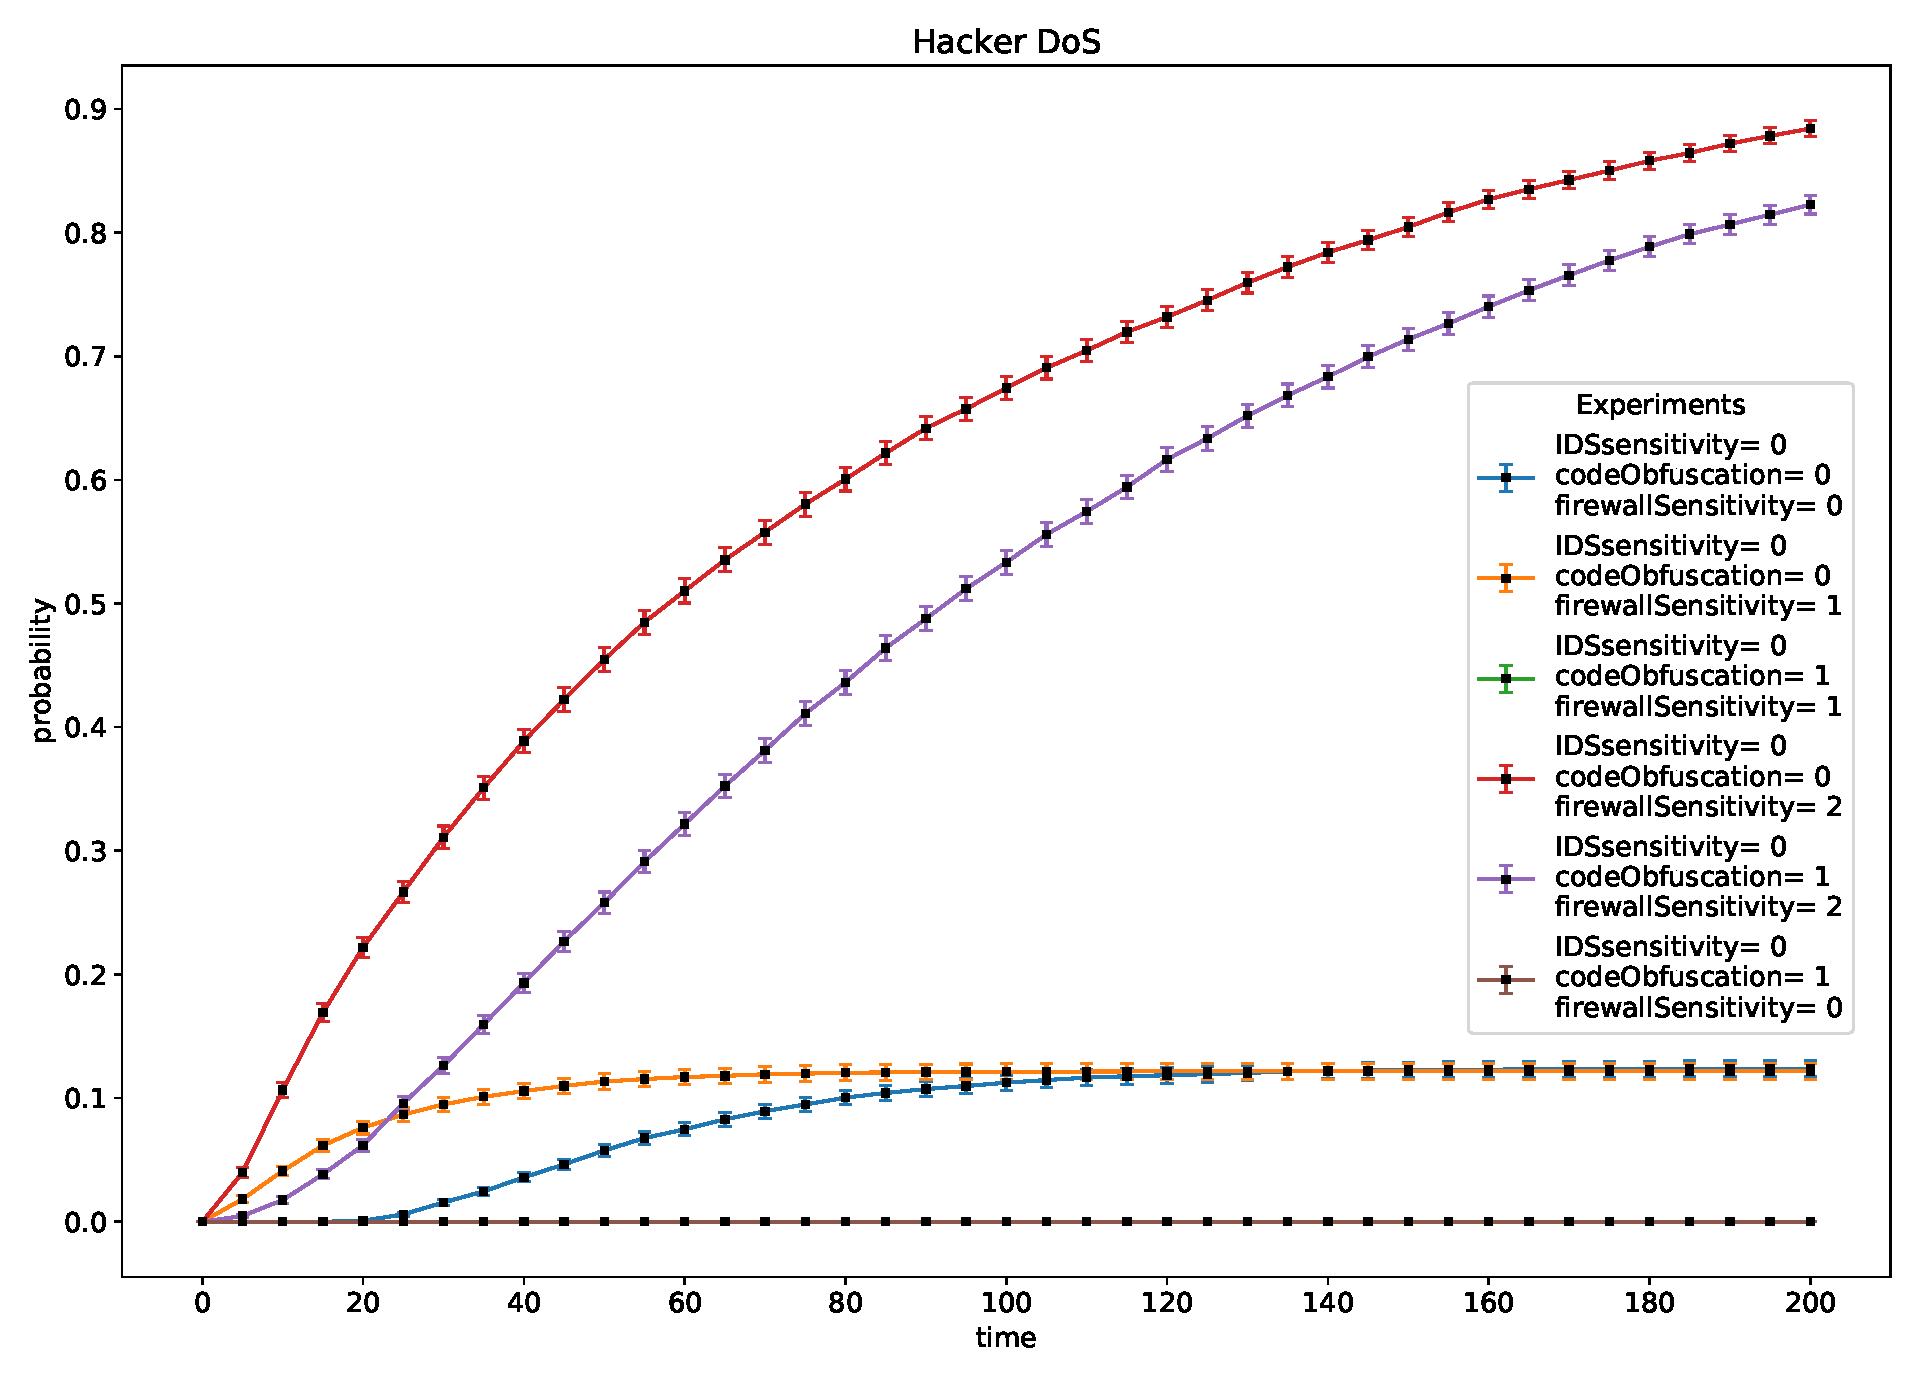
\includegraphics[scale=0.45]{img/Hacker_DoS.pdf}
    \end{center}
    \caption{Hacker DoS}
    \label{fig:Hacker_DoS}
    \vspace*{-0.8cm}
\end{figure}
\newpage
\subsection*{Data Breach and Vehicle Undesidered Behaviour}
When no mitigations are applied, the Hacker will reach these goals pretty fast. Introducing \textbf{CodeObfuscation}
will slow them down, but increasing \textbf{Firewall Sensitivity} we are able to reduce their will to reach them
until they will give up. 
\begin{figure}[H]
    \begin{center}
        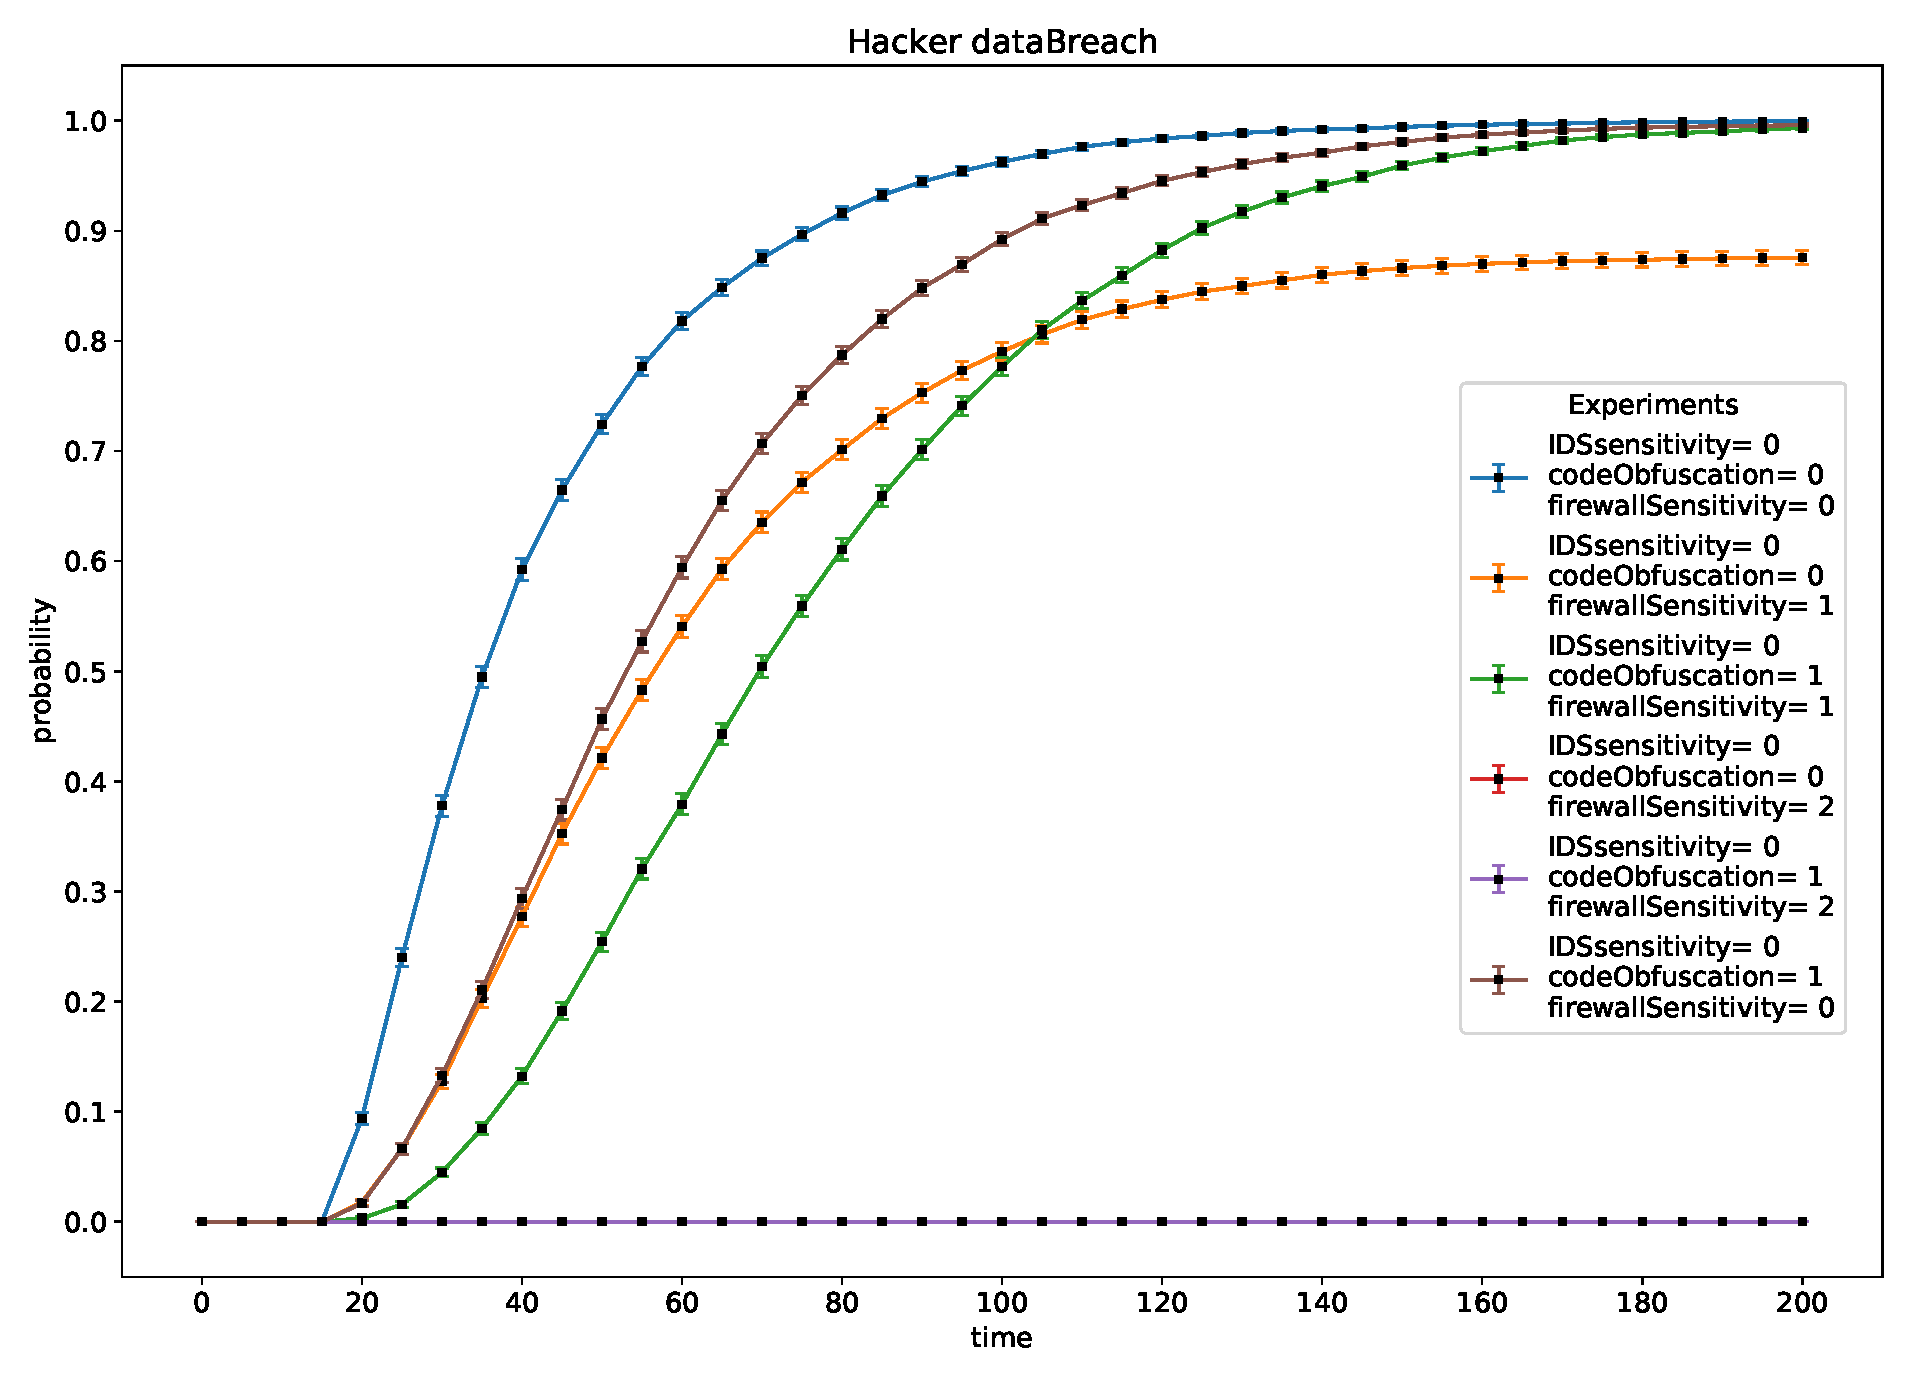
\includegraphics[scale=0.4]{img/Hacker_dataBreach.pdf}
        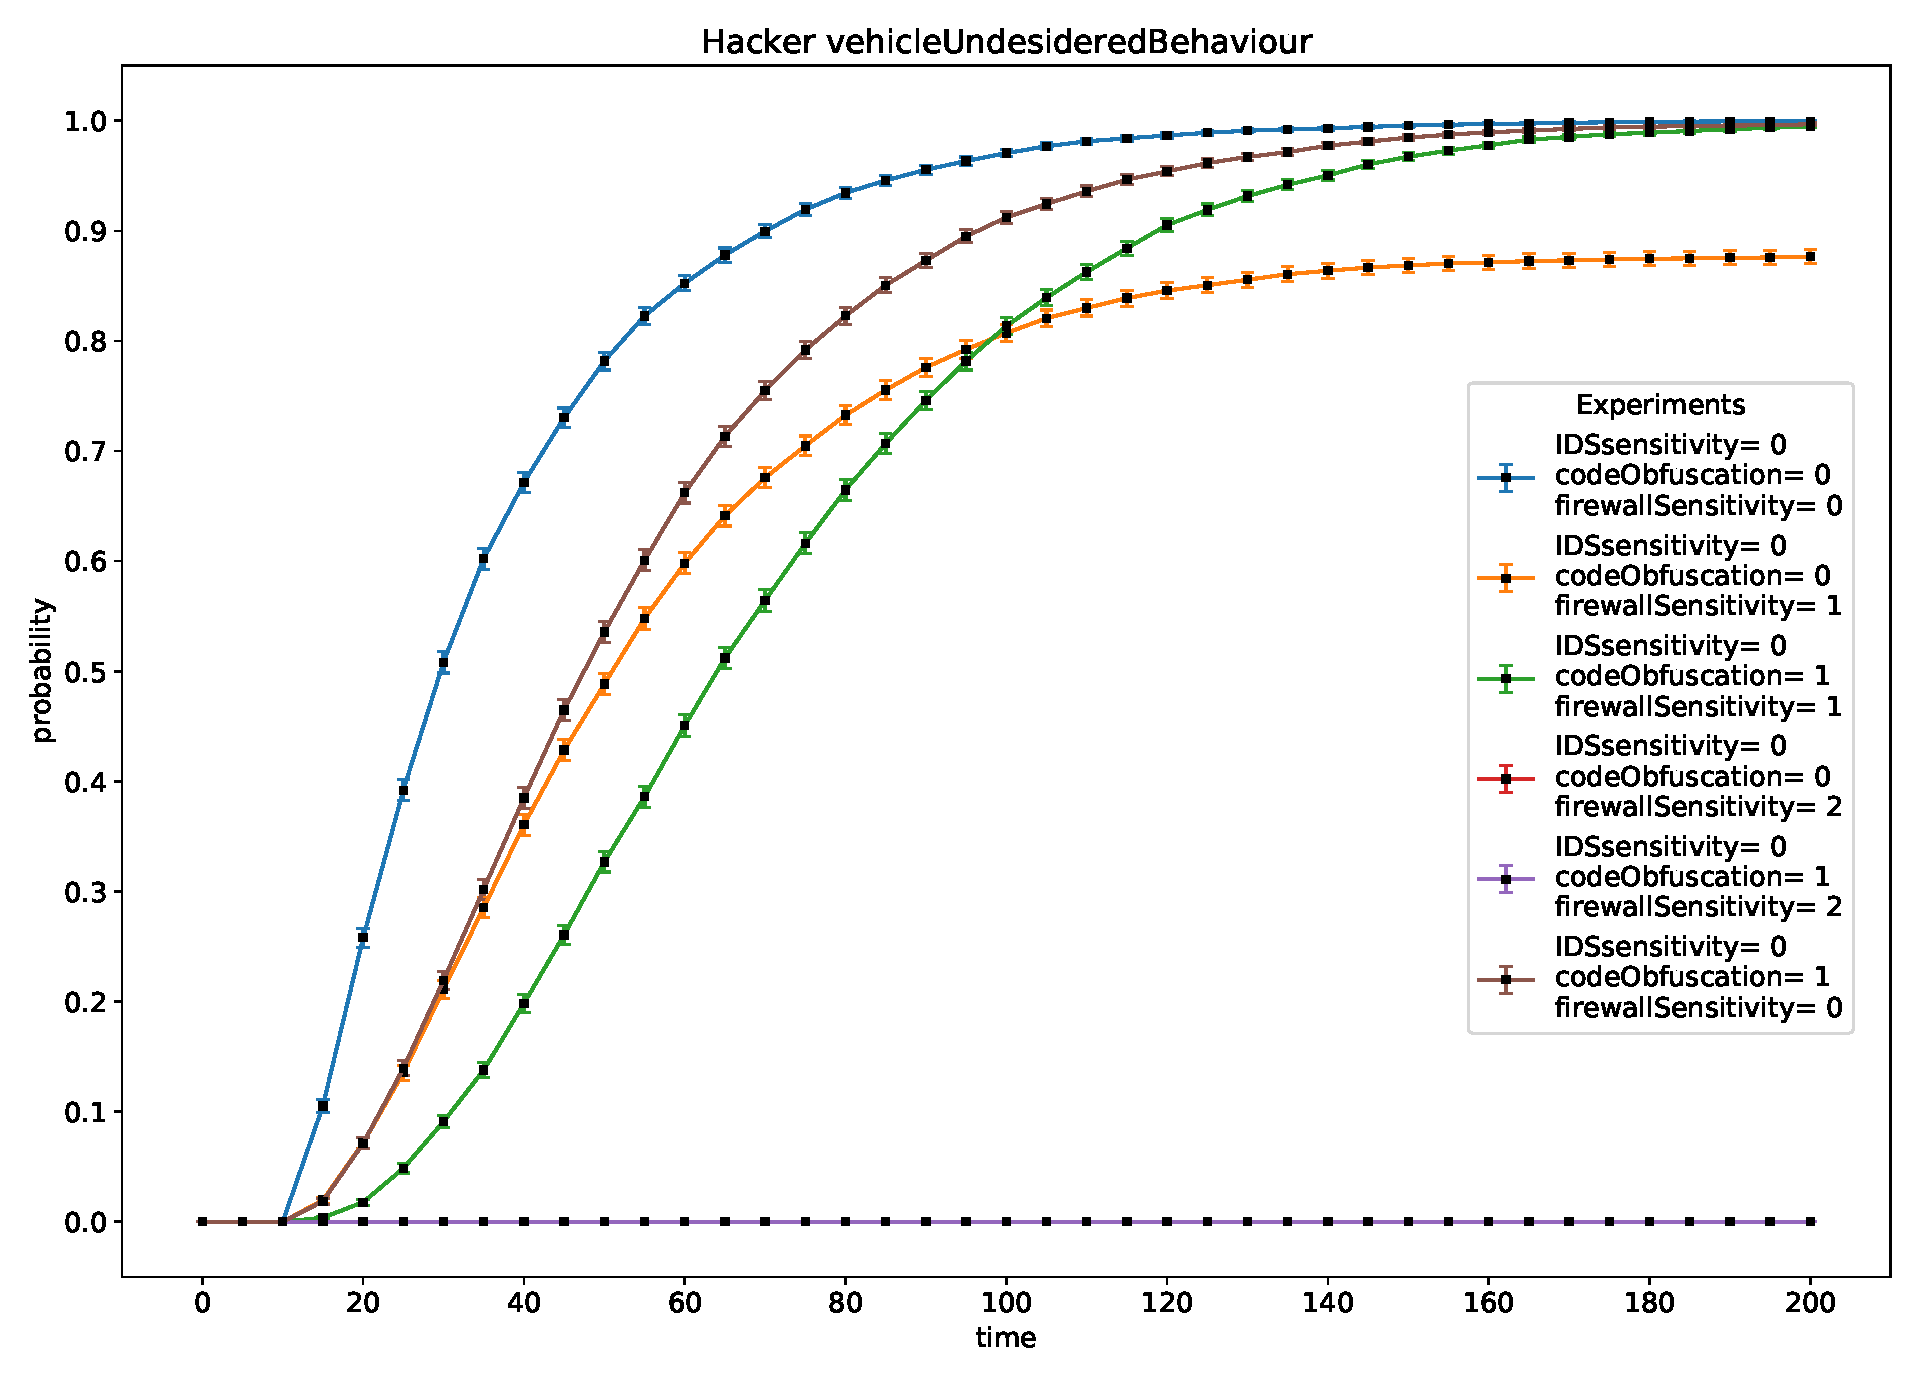
\includegraphics[scale=0.4]{img/Hacker_vOB.pdf}
    \end{center}
    \caption{Hacker Data Breach and Vehicle Undesidered Behaviour}
    \label{fig:Hacker_dataBreach}
    \vspace*{-2cm}
\end{figure}
\section{Physical Intruder and Insider Attacks}

\subsection*{Vehicle Undesired Behaviour}
When no mitigations are applied, both attackers will reach this goal pretty fast. Increasing 
\textbf{Intrusion Detection System Sensitivity}, we are able to reduce their will to reach the goal
until they will give up, because the probability to be discovered will be to high.
\begin{figure}[H]
    \begin{center}
        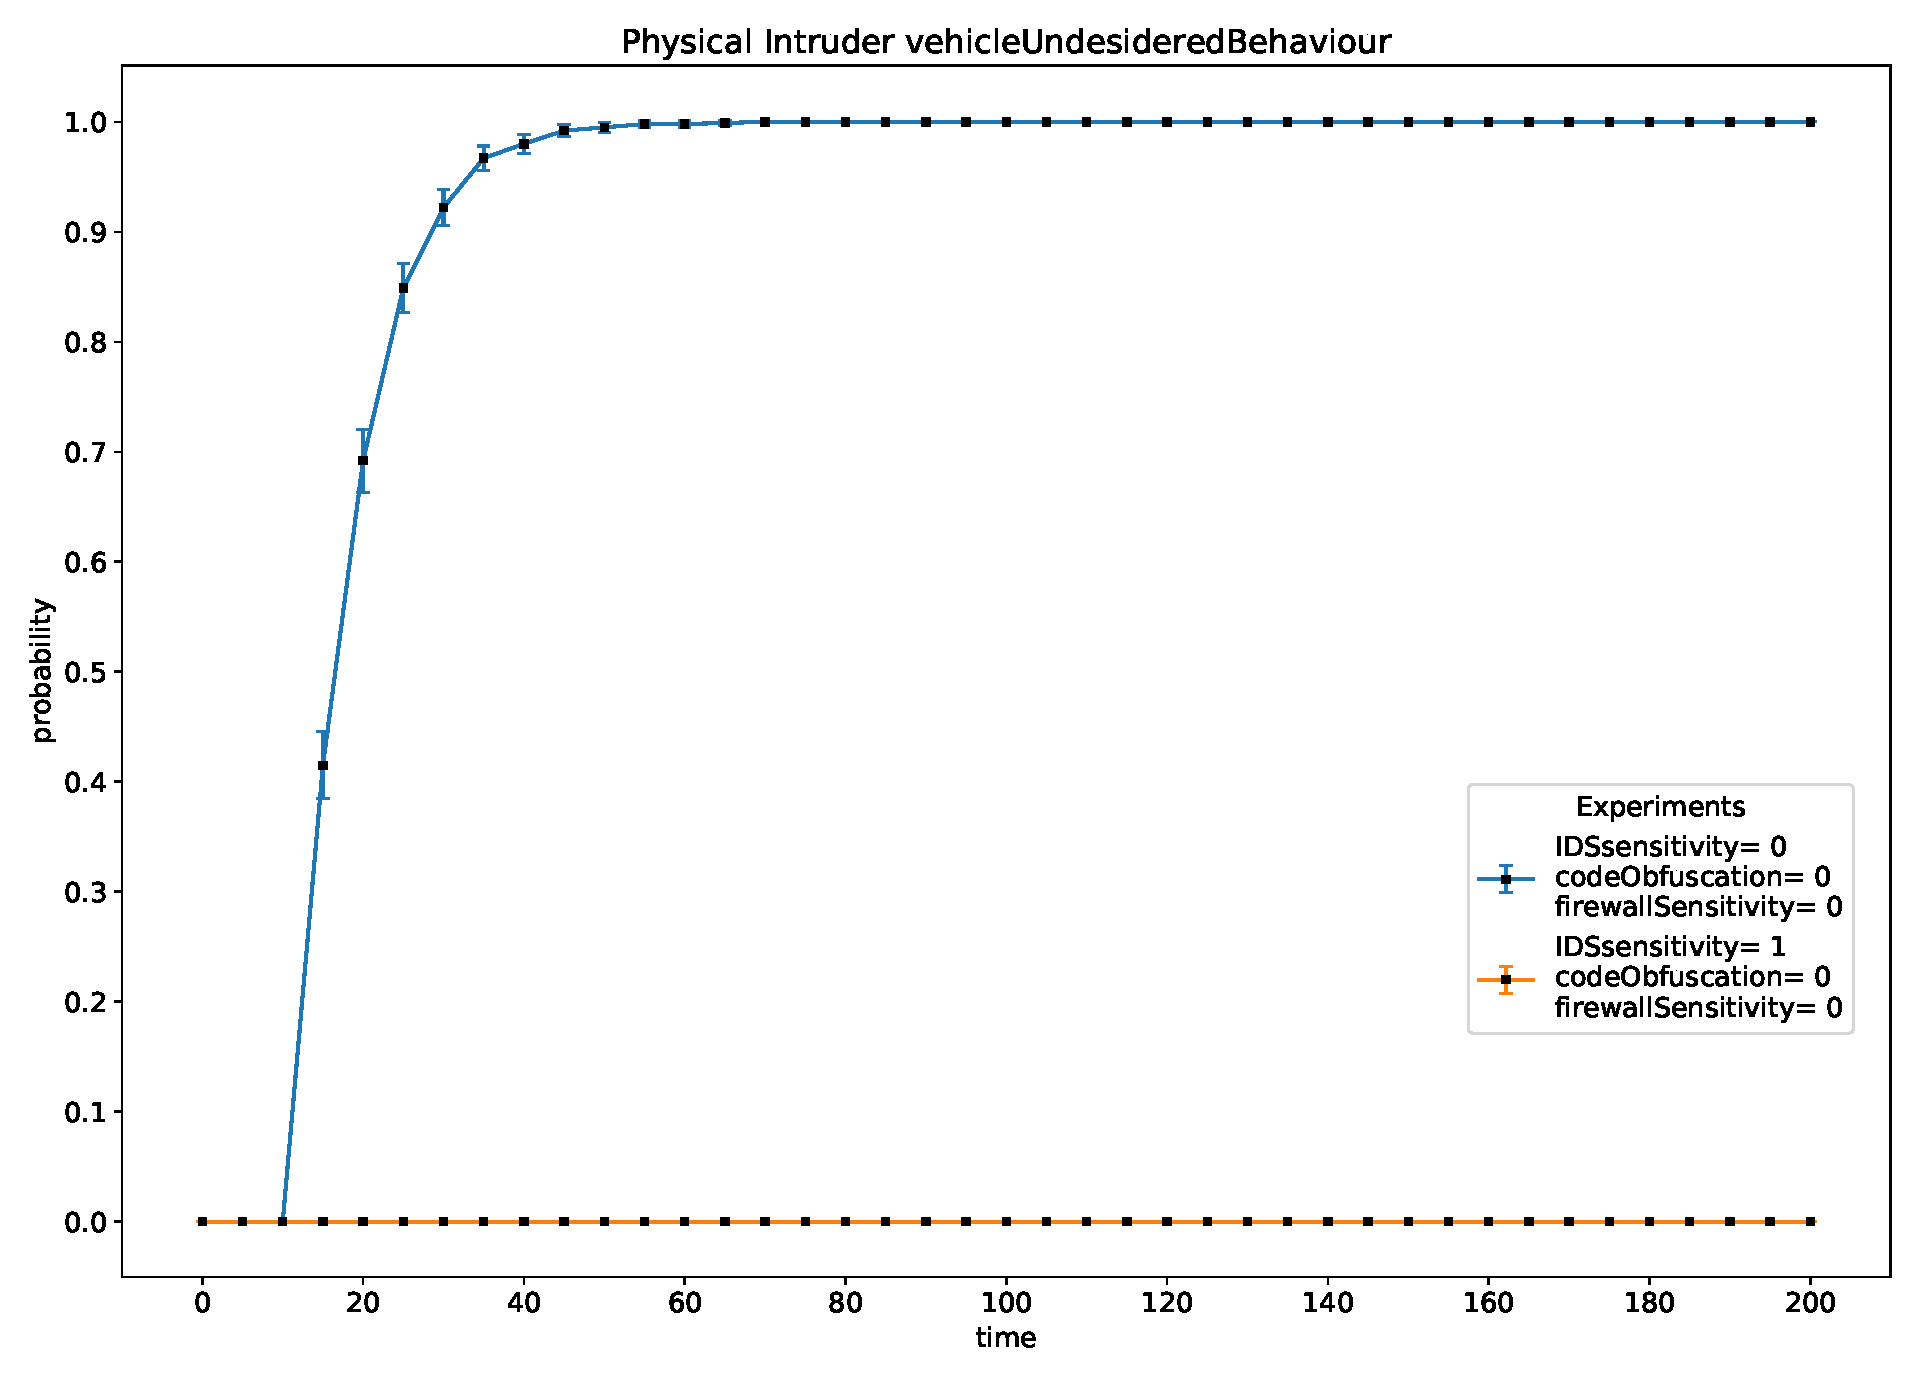
\includegraphics[scale=0.38]{img/Physical_vOB.pdf}
        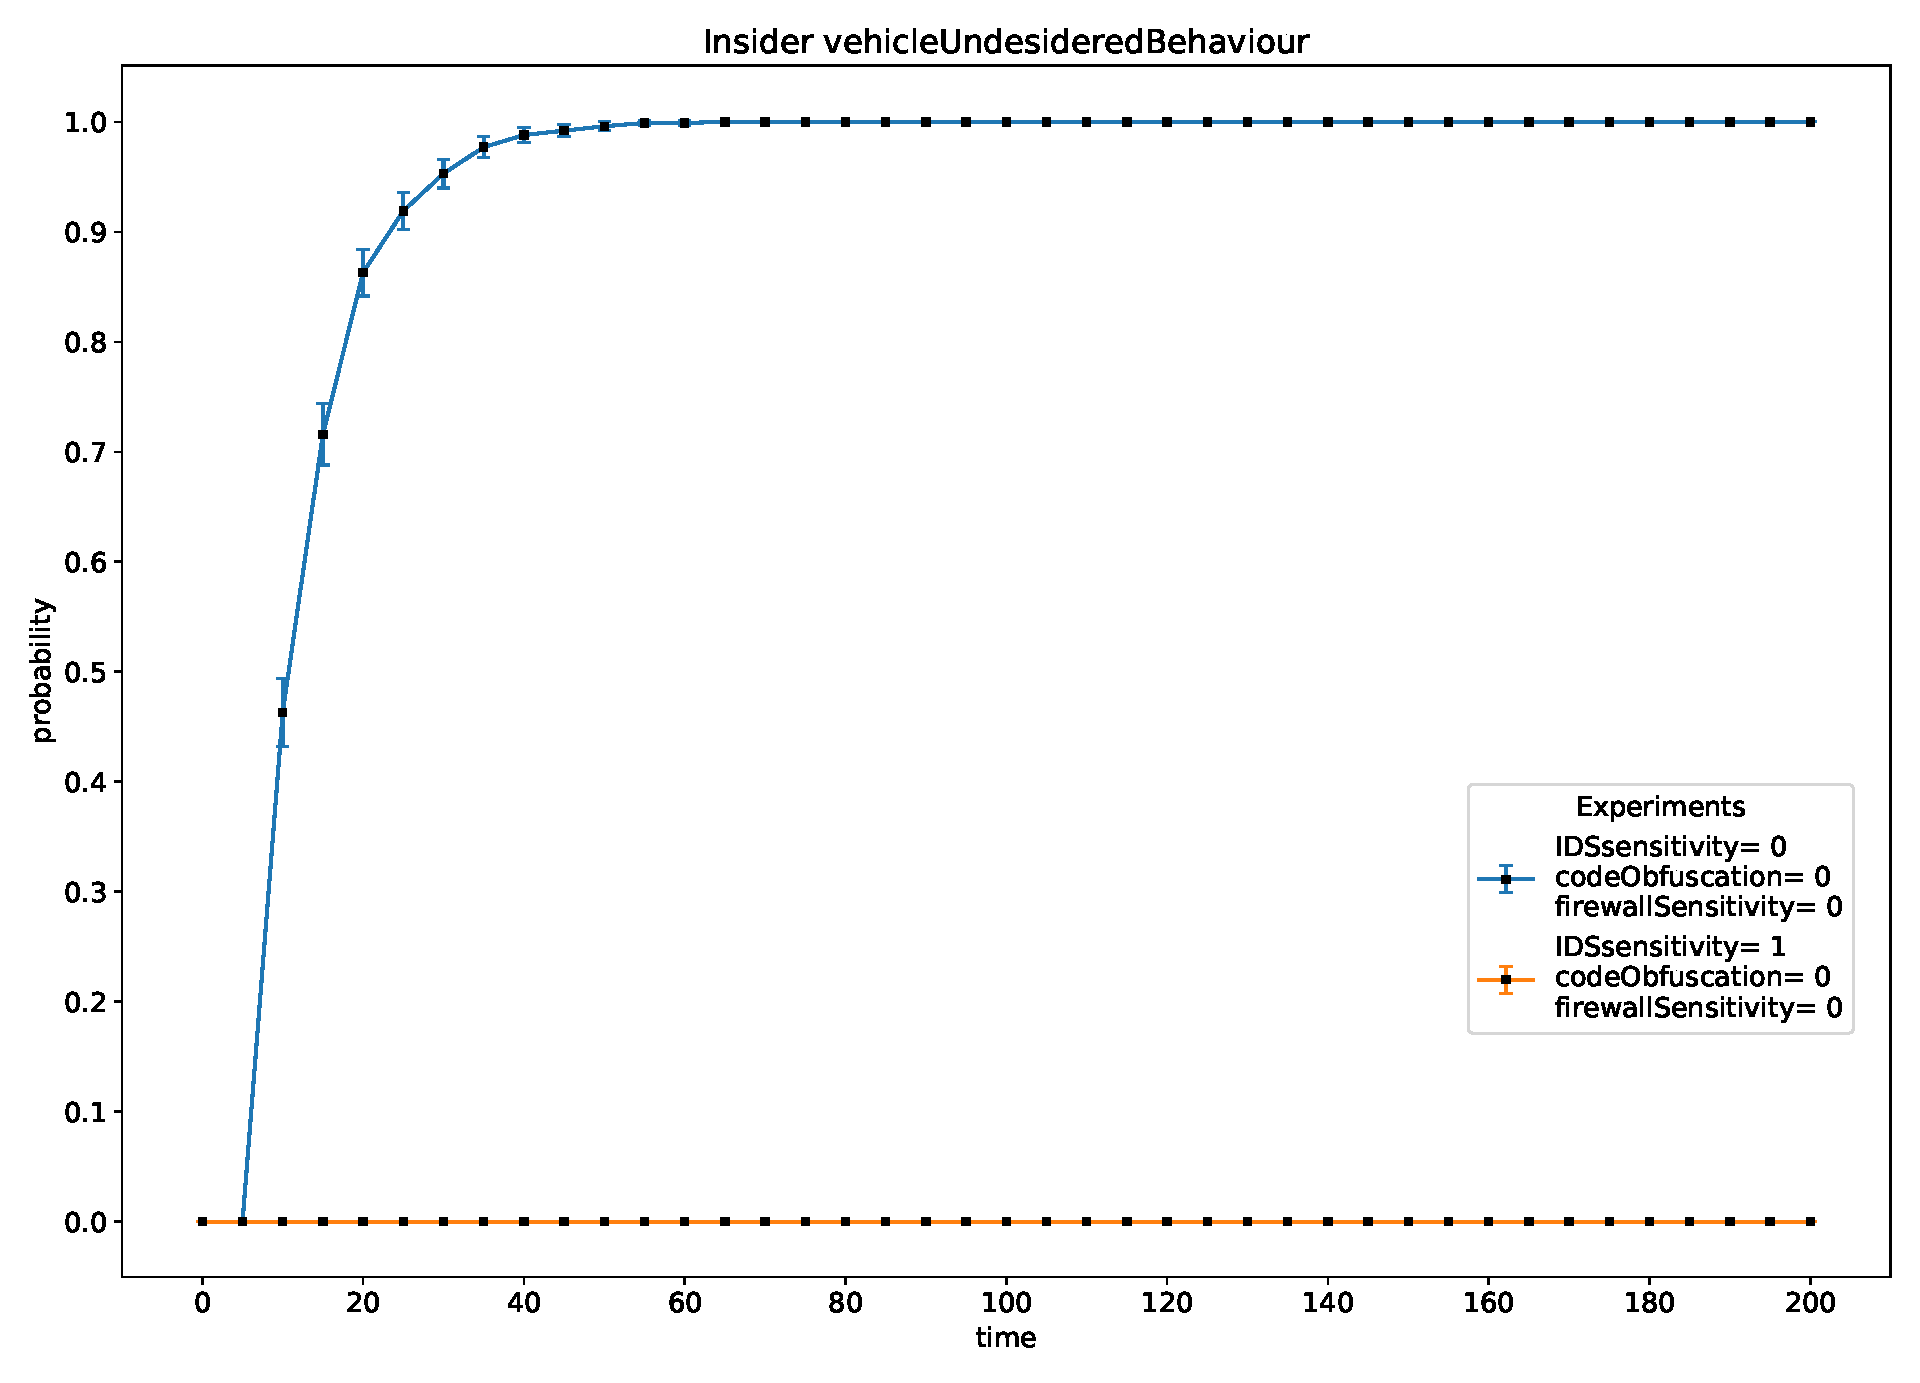
\includegraphics[scale=0.38]{img/Insider_vOB.pdf}
    \end{center}
    \caption{Physical intruder and Insider Vehicle Undesidered Behaviour}
    \label{fig:P_I_vob}
    \vspace*{-3cm}
\end{figure}

It is important to underline that in the case of an insider attacker, the time needed to achieve a high probability is lower w.r.t. the one needed for a physical intruder, since the two attackers follow different paths and the one taken by the physical intruder is longer and requires more time.

\section{Conclusion}
\noindent At the end of our analysis we can infer that is a very good idea to invest in a highly reliable and effective \textbf{Firewall} in order to discourage attacks from the hacker; furthermore IDS and code obfuscation techniques proved to be good countermeasures too.
Therefore implementing these mitigations results in an improvement in the overall security of the system.
